\documentclass[11pt,a4paper]{article}
\usepackage[utf8]{inputenc}
\usepackage[T1]{fontenc}
\usepackage[a4paper,
left=3cm,
top=2cm,
right=1.5cm,
bottom=2cm,
marginparsep=7pt,
marginparwidth=.6in]{geometry}
\usepackage{pscyr}
\usepackage{indentfirst}
\usepackage{mathtext}
\usepackage{amsmath}
\usepackage{amsfonts}
\usepackage{amssymb}
\usepackage[english,russian]{babel}
\RequirePackage{mathtext,amsmath,amssymb,latexsym}
\usepackage{wrapfig}
\usepackage{graphicx}
\usepackage{float}
\begin{document}
	\setcounter{page}{2}
	\tableofcontents
	\newpage
	\section{Цель работы}
	\begin{enumerate}
		\item Экспериментальная проверка уравнения состояния идеального газа.
		\item Определение температуры абсолютного нуля по шкале Цельсия.
	\end{enumerate}
    \section{Теоретические основы лабораторной работы}
    В том случае, когда состояние газа далеко от области фазовых превращений, его с
    достаточной степенью точности можно считать идеальным. В качестве идеального газа в работе
    используется обычный атмосферный воздух.
    
    Для произвольной массы m идеального газа справедливо следующее уравнение состояния
    \begin{equation}
    	pV = \frac{m}{\mu}RT \quad ,
    \end{equation}
    где $ p $ -- давление, $ V $ -- объём, $ \mu $ -- молярная масса, $ T$ -- абсолютная температура газа, $ R $ --
    универсальная газовая постоянная. Это уравнение называется уравнением Менделеева--Клапейрона.
    
    Нулю абсолютной температуры по шкале Цельсия соответствует значение $ t_* = -273,15 ^\circ C$.
    Градусы шкалы абсолютной температуры (шкалы Кельвина) и шкалы Цельсия выбраны
    одинаковыми. Поэтому значение абсолютной температуры связано со значением температуры
    по шкале Цельсия формулой
    \begin{equation}
    	T(K) = t(^\circ C) - t_* = t(^\circ) + 273,15^\circ C \quad .
    \end{equation}
    
Пусть исследуемый газ находиться в цилиндре с контролируемым рабочим объемом $V_ц$ (см.
Рис. 1), масса газа в цилиндре $m_ц$ . Температура $t$ цилиндра с газом поддерживается постоянной. Датчик давления, работающий при комнатной температуре, вынесен за пределы рабочего объема и соединен с последним трубкой. Объем газа $V_х$ в этой трубке мал по сравнению с рабочим объемом $V_ц$ . В соединительной трубке также находится газ массой $m_x$ при некоторой неизвестной средней температуре $t_х$ , лежащей в интервале от комнатной температуры до температуры $t$ рабочего объема.

\begin{wrapfigure}{l}{0.31\textwidth}
	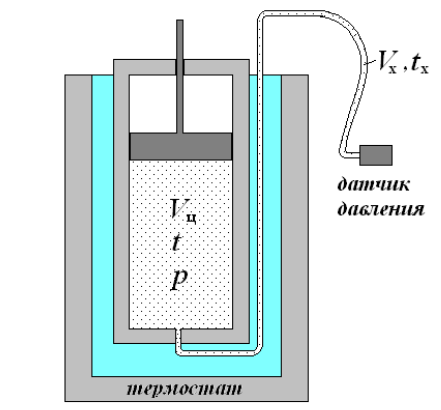
\includegraphics[width=0.3\textwidth]{../im1.png}
	\caption{}
\end{wrapfigure}

В работе измеряется зависимость давления p газа от
величины рабочего объема $V_ц$ при разных значениях
температуры $t$ (от $20^\circ С$ до $60^\circ С$). Выведем соотношение,
связывающее рабочий объем и давление газа при постоянной
температуре. Общее количество вещества в рабочем объеме и
соединительной трубке
\begin{equation}
	\nu = \frac{(m_ц + m_х)}{\mu}
\end{equation}
в течение всей работы остается постоянным. Выражая массы газа m ц и m x из уравнения
состояния (1), абсолютную температуру из соотношения (2), и подставляя найденные
выражения в формулу (3), получим
\begin{equation}
	\nu = \frac{pV_ц}{R(t - t_*)} + \frac{pV_х}{R(t - t_*)} \quad .
\end{equation}

Из этого уравнения найдем искомое соотношение:
\begin{equation}
	V_ц = \frac{\nu R(t - t_*)}{p} - \frac{V_х(t - t_*)}{(t_х - t_*)} \quad .
\end{equation}

Из-за перераспределения газа между объемами $V_ц$ и $V_х$ в процессе измерения температура $t_х$
может изменяться. Однако, при относительно малой величине $V_х$ изменением второго
слагаемого в формуле (5) можно пренебречь. Поэтому при неизменной температуре $t$
зависимость рабочего объема $V_ц$ от обратного давления $1/p$ является линейной. Угловой
коэффициент этой зависимости
\begin{equation}
	K = \mu R(t - t_*)
\end{equation}
в свою очередь, линейно меняется с температурой и обращается в нуль при абсолютном нуле
температур. Таким образом, изучение зависимости $K(t)$ позволяет найти значение $t_*$ .

Рассмотрим другой, более точный, способ определения величины $t_*$ . Если для разных
температур измерение давления проводить при одних и тех же значениях объема, то
полученные данные легко преобразуются в зависимость давления от температуры при разных
значениях рабочего объема газа. Теоретический вид этой зависимости получается из уравнения
(5) :
\begin{equation}
	p =\frac{\nu R(t-t_*)}{V_ц(1+x(t))} \approx \frac{\nu R(t-t_*)}{V_ц} \quad ,
\end{equation}
где $x(t) = \frac{V_х(t-t_*)}{V_ц(t_x - t_*)}$ . Справедливость приближенного равенства в формуле (7) обусловлена тем, что значения функции $x(t)$ малы, и для малых $x$ можно воспользоваться формулой приближен-
ных вычислений:
\begin{equation}
	(1+x)^\alpha \approx 1 + \alpha x
\end{equation}
В данном случаем $\alpha = -1$.
При неизменном рабочем объеме $V_ц$ график зависимости давления от температуры в
соответствии с формулой (7) должен быть почти линейным. Причем давление должно
обращаться в нуль как раз при $t = t_*$ . Из-за малости функции $x(t)$ отклонение от линейности
невелико, и при измерении в ограниченном диапазоне температур практически незаметно. Но,
если искать значение $t_*$ с помощью линейной аппроксимации экспериментальной зависимости
$p(t)$ , продолжая (экстраполируя) аппроксимирующую прямую до пересечения с осью $t$, то
найденное приближенное значение $\widetilde{t_*}$ окажется систематически смещенным влево относительно
истинного значения $t_*$ (см. Рис. 2). Причина этого в следующем. Величина $x(t)$ в первом
приближении линейно растущая функция температуры, с учетом этого график функции $p(t)$ из
\begin{wrapfigure}{l}{0.31\textwidth}
	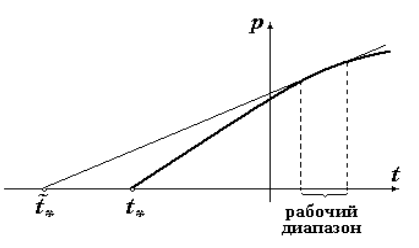
\includegraphics[width=0.3\textwidth]{../im2.png}
	\caption{Жирная линия -- экстраполяция реальной параболической зависимости, обычная линия -- экстраполяция с
		помощью аппроксимирующей
		прямой, проведенной по точкам в
		рабочем диапазоне температур.}
\end{wrapfigure}
уравнения (7) оказывается параболой выпуклой вверх.
Аппроксимирующая прямая, параметры которой найдены
по точкам в рабочем диапазоне температур, идет
практически по касательной к этому графику,
«промахиваясь» мимо истинного значения $t_*$ , как
изображено на Рис. 1. Однако, можно показать, что
разность $\widetilde{t_*} - t_*$ при малом отношении $V_x/V_ц$ должна
убывать обратно пропорционально объему $V_ц$ . Поэтому,
правильное значение температуры абсолютного нуля
\begin{equation}
	t_* = \lim\limits_{1/V_ц \to 0} \widetilde{t_*} \quad ,
\end{equation}
линейным продолжением графика зависимости $t_*$ от $V_ц$
к значению $V_ц =0$ .
~\\\\\\\\
\newpage
\section{Протокол измерений}
\newpage
\section{Задание 1}
Для каждой из таблица 1.1 -- 1.5 вычислить давление газа $p$ по формуле
\begin{equation}
	p = p_0 + \frac{\Delta p_1 + \Delta p_2}{2}
\end{equation}
обратное давление $1/p$ и заполнить пятую и шестую колонки таблиц.
\section{Задание 2}
По данным таблиц 1.1 -- 1.5 для температур $t_1 , t_2 ...  t_5$ построить на одной координатной сетке
графики зависимости рабочего объема $V_ц$ от обратного давления $1/p$ . Убедится, что
зависимость $V_ц$ от $p$ во всех пяти случаях является прямолинейной.

График 1 приведён в Приложении 1. Зависимости линейные.
\section{Задание 3}
Перенести значения рабочих температур $t_1 , t_2 ...  t_5$ во второй столбец таблицы 2.1. Для
каждого из графиков $V_ц$ от $1/p$ рассчитать угловой коэффициент $K$ по МНК. Построить теоретическую зависимость $K(t)$. По найденным экспериментальным точкам найти угловой коэффициент $A$ и
свободное слагаемое $C$ для зависимости $K(t)$. Рассчитать
температуру абсолютного нуля:
\begin{equation}
	t_* = - \frac{C}{A}
\end{equation}
найти погрешности $A$ и $C$ и вычислить погрешность
температуры абсолютного нуля:
\begin{equation}
	\Delta t_* = t_* \sqrt{\left(\frac{\Delta A}{A}\right)^2 + \left(\frac{\Delta C}{C}\right)^2}
\end{equation}
\begin{table}[H]
	\renewcommand\thetable{1.1}
	\caption{Зависимость углового коэффициента графика $V_ц(1/p)$ от температуры газа}
	\centering
	\begin{tabular}{|c|c|c|}
		\hline
		№ п.п. & t, $^\circ C$, & $К$, Дж\\
		\hline
		1 & $16,5$ & $8707$\\
		\hline
		2 & $32,6$ & $9035$\\
		\hline
		3 & $44,1$ & $9308$\\
		\hline
		4 & $50,1$ & $9486$\\
		\hline
		5 & $59,2$ & $9759$\\
		\hline
	\end{tabular}

\begin{equation}
	A = (24,4 \pm 1,3); \qquad C = (8269 \pm 57); \qquad t_* = (-339 \pm 145)^\circ C
\end{equation}
\end{table}
График 2 $K(t)$ приведён в Приложении 1.
\section{Задание 4}
По данным таблиц 1.1 -- 1.5 заполнить таблицу 2.2. Для каждого из объемов в таблице 2.2 найти значение обратного объема $1/V_ц$ и
рассчитать величину $t_*$.

Пользуясь таблицей 2.2 для значений объема цилиндра 50, 90, 120 мл на одной
координатной сетке построить графики $p(t)$ , убедится, что они «идут» прямолинейно.
с угловым коэффициентом $A'$ и свободным слагаемым $C'$.
Используя таблицу 2.2 построить зависимость $\widetilde{t_*}(1/V_ц)$
\begin{figure}[H]
	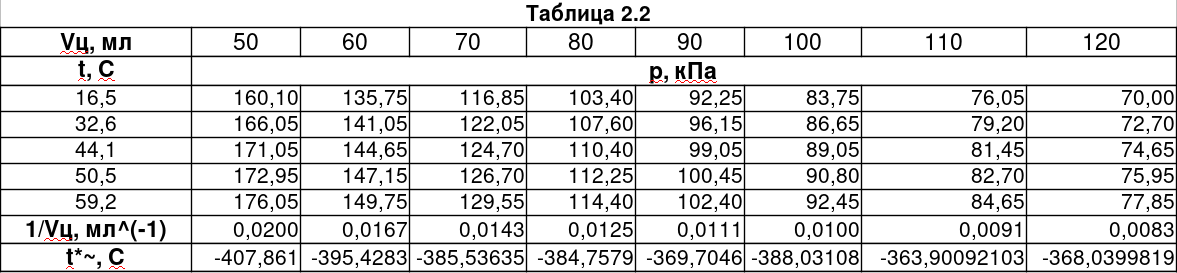
\includegraphics[scale=0.38]{../t.png}
\end{figure}
Зависимости $p(t)$ для 50, 90 и 120 мл приведены в Графике 3 Приложении 1.

\begin{equation}
A' = (3310 \pm 690); \quad C' = (-340.7 \pm 9,2)
\end{equation}

Зависимость $\widetilde{t_*}(1/V_ц)$ приведена в Графике 4 в Приложении 1.
\section{Вывод}
В ходе этой лабораторной работы я рассчитал температуру абсолютного нуля двумя способами. Через график $K(t)$ $(-339 \pm 145)^\circ C$ и через $\widetilde{t_*}(1/V_ц)$  $(-340.7 \pm 9,2)^\circ C$. Первое близко к табличному значению с учетом погрешности.
\end{document}